\documentclass[11pt,a4paper]{article}
\usepackage[margin=2.3cm]{geometry}
\usepackage[T1]{fontenc}
\usepackage{mathptmx}
\usepackage{microtype}
\usepackage{amsmath,amssymb}
\usepackage{graphicx}
\usepackage{booktabs}
\usepackage{caption}
\usepackage[hidelinks]{hyperref}
\captionsetup{font=small,labelfont=bf}
\setlength{\parskip}{0.35em}
\newcommand{\TabQuality}{uniform random $k$-subset & 1 & 0.653 [0.626, 0.678] & 0.011 [0.007, 0.016] & 0.726 [0.708, 0.746] \\
penalty, $P_{\rm auto}$ & 0.57 & 0.653 [0.627, 0.679] & 0.006 [0.004, 0.009] & 0.727 [0.709, 0.746] \\
penalty, $P_{\rm tight}$ & 0.55 & 0.659 [0.633, 0.685] & 0.007 [0.004, 0.010] & 0.734 [0.717, 0.752] \\
XY, basis start & 1.00 & 0.811 [0.761, 0.859] & 0.029 [0.000, 0.075] & 0.837 [0.799, 0.872] \\
XY, Dicke start & 1.00 & 0.795 [0.771, 0.816] & 0.073 [0.047, 0.102] & 0.826 [0.804, 0.847] \\}
\newcommand{\TabSlopes}{penalty, $P_{\rm auto}$ & $-0.15$ [$-0.22$, $-0.09$] & $0.22$ [$0.15$, $0.29$] \\
penalty, $P_{\rm tight}$ & $-0.15$ [$-0.21$, $-0.08$] & $0.06$ [$-0.05$, $0.15$] \\
XY, basis start & $-0.18$ [$-0.29$, $-0.08$] & $-0.16$ [$-0.25$, $-0.09$] \\
XY, Dicke start & $-0.15$ [$-0.23$, $-0.09$] & $-0.10$ [$-0.20$, $-0.02$] \\
RealAmplitudes (HEA) & $-0.18$ [$-0.20$, $-0.15$] & $-0.30$ [$-0.31$, $-0.28$] \\}
\newcommand{\TabCost}{8 & 123 / 52 (2.34) & 249 / 112 (2.23) & 379 / 179 (2.11) \\
10 & 209 / 133 (1.57) & 424 / 294 (1.44) & 634 / 464 (1.37) \\
12 & 310 / 137 (2.27) & 625 / 290 (2.15) & 948 / 454 (2.09) \\
14 & 429 / 205 (2.09) & 875 / 466 (1.88) & 1328 / 717 (1.85) \\}
\newcommand{\TabHW}{penalty, $p=1$ & 13 & 12.3 [11, 13] & 0.12 & 0.74 & 0.187 & 0.184 \\
XY (basis), $p=1$ & 9 & 6.0 [6, 6] & 1.00 & 0.46 & 0.765 & 0.825 \\
penalty, $p=2$ & 12 & 10.9 [8, 12] & 0.50 & 0.63 & 0.127 & 0.126 \\
XY (basis), $p=2$ & 10 & 8.0 [8, 8] & 0.99 & 0.62 & 0.604 & 0.652 \\
penalty, $p=3$ & 11 & 11.3 [11, 12] & 0.87 & 0.69 & 0.212 & 0.210 \\
XY (basis), $p=3$ & 11 & 11.8 [10, 12] & 0.87 & 0.62 & 0.427 & 0.434 \\}
\newcommand{\NR}{72}
\newcommand{\NH}{12}
\newcommand{\HardRate}{0.3}
\newcommand{\DickeWins}{252}
\newcommand{\DickeTot}{252}
\newcommand{\BasisSig}{13}
\newcommand{\BasisTot}{15}
\newcommand{\RandBestK}{0.999}
\newcommand{\PenBestK}{0.996}
\newcommand{\PenTopOne}{0.99}
\newcommand{\NullMean}{11.5}
\newcommand{\GreedyFailR}{3}
\newcommand{\GreedyH}{0.945}
\newcommand{\LPH}{0.928}
\newcommand{\LamSparse}{100.0}
\newcommand{\LamDense}{98.5}
\newcommand{\LamZeroSparse}{4}
\newcommand{\LamZeroDense}{0}
\newcommand{\WsR}{0.834}
\newcommand{\StdR}{0.683}
\newcommand{\WsH}{0.827}
\newcommand{\StdH}{0.733}
\newcommand{\MaStdOne}{$4.4\times10^{-3}$}
\newcommand{\MaStdFortyFive}{$7.9\times10^{-6}$}
\newcommand{\MaOne}{$3.3\times10^{-6}$}

\newcommand{\Pauto}{P_{\rm auto}}
\newcommand{\Ptight}{P_{\rm tight}}

\title{\vspace{-1.2cm}Constraint-native versus penalty QAOA\\ for budgeted maximum coverage:\\ quality, trainability and hardware cost}
\author{F.~Pisaturo\\[2pt]\small University of Salerno \quad \texttt{f.pisaturo2@studenti.unisa.it}}
\date{October 2026}

\begin{document}
\maketitle
\vspace{-0.6cm}
\begin{abstract}
\noindent Budget constraints of the form $\sum_i x_i = k$ can be imposed on the Quantum
Approximate Optimization Algorithm (QAOA) either through a quadratic penalty or structurally,
with a Hamming-weight-preserving XY mixer. I compare the two encodings on a weather-station
placement problem (maximum coverage with $k$ of $n$ stations) for $n=8$--$14$ and depth
$p=1$--$3$, over \NR{} random instances and \NH{} instances on which greedy and LP rounding both
fail. Using exact statevector simulation and identical metrics for all methods, the XY mixer
reaches an expected coverage ratio of about $0.80$ per shot, against $0.66$ for penalty QAOA,
which is statistically indistinguishable from sampling uniformly random feasible subsets. The
cost variance over random parameters decays at the same rate for both encodings, so the gap is
not a trainability effect. After routing to the heavy-hex coupling map of \texttt{ibm\_marrakesh},
penalty QAOA needs about twice as many two-qubit gates. A re-analysis of an earlier hardware run
shows that its reported statistic cannot distinguish the circuits from uniform noise. At these
sizes the problem is classically trivial; the study compares encodings, not quantum and classical
solvers.
\end{abstract}

\section{Introduction}
Many combinatorial problems of practical interest carry hard constraints. In QAOA~\cite{farhi2014}
the usual route is to fold them into the cost as a penalty and keep the transverse-field mixer.
The alternative proposed by Hadfield et al.~\cite{hadfield2019} is to choose a mixer that commutes
with the constraint and to start from a feasible state, so that the circuit never leaves the
feasible subspace. The second option removes the penalty weight as a hyperparameter and wastes
no shots on infeasible strings, but it changes the circuit and the optimisation landscape.

This report asks which encoding is preferable for a cardinality constraint, using three
criteria: (i) solution quality at fixed depth, (ii) trainability, measured by how concentrated
the cost is over random parameters~\cite{mcclean2018,arrasmith2022}, and (iii) gate cost after
routing to a real device. The test problem is the placement of $k$ weather stations among $n$
candidates so as to cover as many zones as possible (maximum coverage).

The contributions are modest in scope and are stated with that in mind:
\begin{itemize}\setlength\itemsep{0pt}
\item a controlled comparison with identical metrics and optimiser budgets, over \NR{}+\NH{}
instances with confidence intervals and paired tests;
\item the observation that two common metrics, the most probable bitstring and the best of
$\sim$1000 shots, hide the difference between the encodings at this size;
\item a gate-count comparison after routing, and a fair re-analysis of one hardware run.
\end{itemize}
At $n\le 14$ exhaustive enumeration solves every instance instantly, so nothing here bears on
quantum advantage.

\section{Problem and encodings}
\paragraph{Maximum coverage and its QUBO proxy.} Station $i$ covers the zone set $A_i$; we seek
$x\in\{0,1\}^n$, $\sum_i x_i=k$, maximising $f(x)=|\bigcup_{i:x_i=1}A_i|$. The exact integer program
needs one variable per zone; a QUBO built from it would need slack qubits for every linking
inequality. QAOA therefore optimises the proxy
\begin{equation}
g_\lambda(x)=\sum_i c_i x_i-\lambda\sum_{i<j} o_{ij}x_ix_j,\qquad c_i=|A_i|,\; o_{ij}=|A_i\cap A_j|,
\end{equation}
which is inclusion--exclusion truncated at second order. A zone covered by $m$ selected stations
contributes $m-\lambda\binom{m}{2}$ to $g_\lambda$ and 1 to $f$. For $\lambda=1$ the proxy is exact when
$m\le2$ and, by the Bonferroni inequalities, $g_1\le f$ in general; it under-counts zones covered
three or more times. Over 200 instances per density class ($n=12$, $k=4$), the maximiser of $g_1$
is a true optimum in \LamSparse\% (sparse) and \LamDense\% (dense) of cases, against
\LamZeroSparse\% and \LamZeroDense\% without the overlap term; values of $\lambda$ away from 1
perform worse in both directions. $\lambda=1$ is used throughout, and all results are reported against
the true objective $f$, so proxy errors are included in them.

\paragraph{Penalty encoding.} Penalty QAOA minimises $C_P(x)=-g_1(x)+P(\sum_ix_i-k)^2$. Two values
of $P$ are compared. $\Pauto=1+\sum_i c_i+\sum_{i<j}o_{ij}$ is the default of
\texttt{qiskit-optimization}, a bound on the whole objective range (30--50 here). The second,
\begin{equation}
\Ptight = 1+\Big\lfloor \max_i \max\big(c_i,\;\textstyle\sum_{j\ne i}o_{ij}-c_i\big)\Big\rfloor ,
\end{equation}
is the smallest value covered by a simple argument that every minimiser is feasible. From a
selection with $k+t$ stations, removing one changes $-g_1$ by at most $c_i$ while the penalty
falls by $P(2t-1)\ge P$. From $k-t$ stations, adding one changes $-g_1$ by at most
$\sum_j o_{ij}-c_i$ while the penalty falls by at least $P$. The property was also checked by brute
force on every instance.

\paragraph{Ansätze.} Penalty QAOA starts from $|+\rangle^{\otimes n}$ and alternates $e^{-i\gamma_l C_P}$ with
$e^{-i\beta_l\sum_iX_i}$. The constraint-native ansatz alternates $e^{-i\gamma_l C}$, with $C=-g_1$ and
no penalty, with a ring XY mixer applied as one Trotter step,
$\prod_{i}e^{-i\beta_l(X_iX_{i+1}+Y_iY_{i+1})/2}$ (indices mod $n$). Each factor preserves Hamming weight,
so the product does too, independently of Trotter error. Two initial states are used: the basis
state $|1^k0^{n-k}\rangle$ (cheap; used on hardware) and the Dicke state $|D^n_k\rangle$, the uniform
superposition over weight $k$ and the feasible analogue of $|+\rangle^{\otimes n}$. The Dicke state costs
$O(kn)$ two-qubit gates to prepare~\cite{baertschi2019}; that cost is not included in
Section~\ref{sec:cost}.

\section{Methods}
\paragraph{Simulation and validation.} All circuits ($\le 2^{14}$ amplitudes) are simulated exactly
with a small NumPy statevector code that also provides adjoint (reverse-mode) gradients. States
agree with Qiskit's \texttt{Statevector} of the corresponding circuits to $1-F<10^{-9}$, and
gradients agree with Qiskit's \texttt{ReverseEstimatorGradient} to $<10^{-8}$.

\paragraph{Metrics.} From the exact output distribution I report the probability that a shot is
feasible; the expected ratio $f(x)/f^\star$ of a feasible shot; the probability $p_{\rm opt}$ that
one shot is optimal; and the expected best of $S$ shots, with infeasible shots scoring 0. Every
metric is compared with a uniformly random $k$-subset. No shot noise enters the simulated results.

\paragraph{Optimisation.} Each method gets the same COBYLA budget (250 iterations, 4 seeded
restarts). The restart with the lowest energy is kept, never the one with the best coverage. The
encodings have very different cost scales, so $\gamma$ is optimised in units of $\gamma_{\rm scale}/\max_S|a_S|$,
where $a_S$ are the Pauli coefficients of the cost; $\gamma_{\rm scale}$ is chosen per method, by final
energy, on separate calibration instances.

\paragraph{Instances and statistics.} Stations and 25 zones are placed uniformly in a $10\times10$
box. Family R (coverage radius 2.2) has $n\in\{8,10,12,14\}$, $k=\mathrm{round}(n/3)$, with 20/20/20/12
instances. Family H (radius 3.0, $n=12$, $k=4$) is rejection-sampled so that greedy and
deterministic LP rounding both miss the optimum; only \HardRate\% of draws qualify. On family R,
greedy fails on \GreedyFailR{} of \NR{} instances and the LP relaxation is always integral. Intervals
are 95\% percentile bootstraps over instances; method comparisons use paired Wilcoxon tests.

\section{Results}
\subsection{Solution quality}
\begin{table}[htb]\centering\small
\caption{Quality at $p=3$, $n=12$ (mean [95\% CI]). $P_{\rm feas}$ and $p_{\rm opt}$ refer to family R (20
instances); the last column is family H (12 classically hard instances).}
\label{tab:quality}
\begin{tabular}{lcccc}\toprule
 & $P_{\rm feas}$ & $E[f/f^\star\mid\text{feas.}]$, R & $p_{\rm opt}$, R & $E[f/f^\star\mid\text{feas.}]$, H\\\midrule
\TabQuality
\bottomrule\end{tabular}
\end{table}
\begin{figure}[htb]\centering
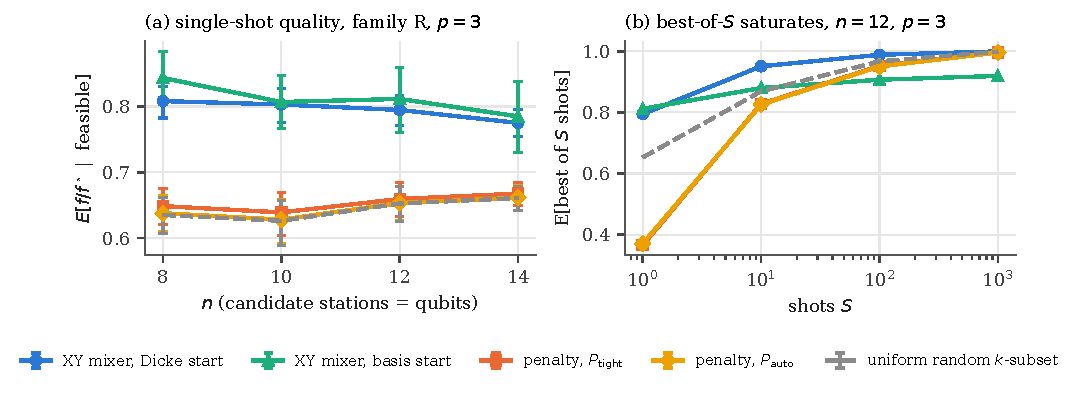
\includegraphics[width=\linewidth]{fig_quality.pdf}
\caption{(a) Expected coverage ratio of a feasible shot vs.\ $n$ (family R, $p=3$, 95\% CI).
(b) Expected best of $S$ shots, infeasible shots counted as 0 ($n=12$). With $\gtrsim100$ shots
uniformly random subsets catch up, so best-of-$S$ metrics cannot separate the methods.}
\label{fig:quality}
\end{figure}
Table~\ref{tab:quality} and Fig.~\ref{fig:quality}a summarise the comparison. Penalty QAOA
is, to within 0.015, a uniform sampler on its feasible shots at every $n$, and its probability of
an optimal shot is \emph{below} that of random subsets. Depending on $n$ and $p$, 35--57\% of its shots
are infeasible. $\Ptight$ improves on $\Pauto$ on almost every instance, but only by about 0.005--0.011. The
XY mixer is better in every setting. With the Dicke start it beats penalty QAOA on \DickeWins{}
of \DickeTot{} paired comparisons over all $(n,p)$. With the basis start the mean gain is similar
and is significant ($p<0.05$) in \BasisSig{} of \BasisTot{} settings, but $p_{\rm opt}$ collapses
with $n$: a few ring layers keep the amplitude within a few hops of an arbitrary initial selection.
On family H the ranking is unchanged. There greedy averages \GreedyH{} and LP rounding \LPH{},
while ten shots of the Dicke-start circuit give about 0.957. Randomized LP rounding and simulated
annealing, however, solve almost every H instance.

Two metrics hide this picture (Fig.~\ref{fig:quality}b). The most probable feasible bitstring of
penalty QAOA is usually optimal (ratio \PenTopOne{} at $p=1$), although its distribution is nearly
flat: the mode is real but cannot be resolved with finite shots. And the best of 1000 shots gives
\PenBestK{} for penalty QAOA and \RandBestK{} for uniform random subsets. An earlier version of this
project scored penalty QAOA with the latter (the default output of Qiskit's
\texttt{MinimumEigenOptimizer}) and the XY mixer with its most frequent bitstring, and concluded the
opposite of what is reported here.

\subsection{Trainability}
\begin{figure}[htb]\centering
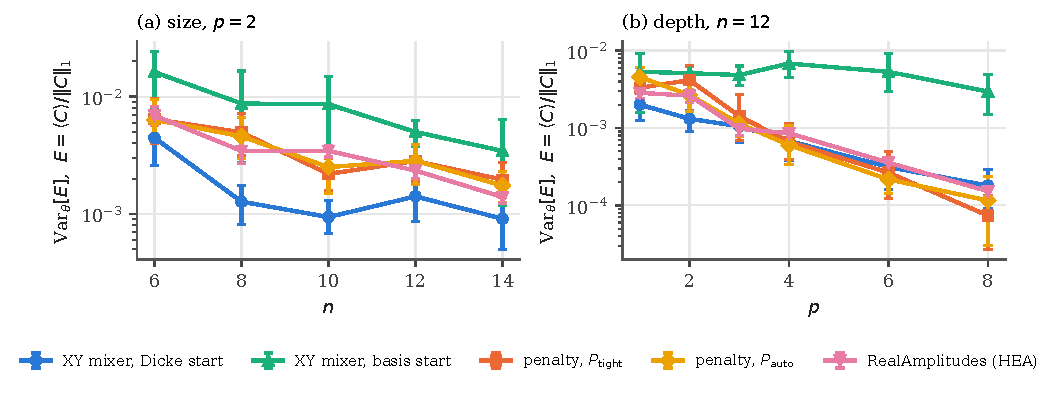
\includegraphics[width=\linewidth]{fig_variance.pdf}
\caption{Variance of the rescaled cost over uniformly random parameters (5 instances $\times$
200 samples per point, 95\% CI). (a) Size scan at $p=2$; (b) depth scan at $n=12$ (120 samples).}
\label{fig:variance}
\end{figure}
\begin{table}[htb]\centering\small
\caption{Fitted slope of $\ln$ variance per qubit, $n=6$--$14$, $p=2$ (95\% bootstrap CI). For
reference, a unitary 2-design gives $-\ln2\approx-0.69$.}\label{tab:slopes}
\begin{tabular}{lcc}\toprule
Ansatz & $\mathrm{Var}_\theta[E]$ & $\overline{\mathrm{Var}}_\theta[\partial_jE]$\\\midrule
\TabSlopes
\bottomrule\end{tabular}
\end{table}
Parameters are drawn uniformly over full periods of the un-rescaled circuit: $\gamma\in[0,2\pi)$,
since all costs have integer spectra; $\beta\in[0,\pi)$ for the transverse mixer; $[0,2\pi)$ for XY hops and
$R_Y$ angles. The measured observable is rescaled, $E=\langle C\rangle/\|C\|_1$ with $\|C\|_1$ the total Pauli weight,
so that $|E|\le1$ for every method; the circuit is not rescaled. I report both the cost variance
and the mean variance of the exact gradient components.

The cost variance decreases with $n$ at the same rate for every ansatz, within overlapping
intervals (Fig.~\ref{fig:variance}a, Table~\ref{tab:slopes}). The rate is several times slower than the
2-design value, so none of these shallow circuits is near a barren plateau at these sizes. Over
$p=1\to8$ the cost variance falls by a factor of 10--45 for penalty QAOA, the Dicke-start XY mixer and the
hardware-efficient ansatz. For the basis-start XY mixer it stays nearly flat, consistent with its
amplitude remaining near the initial state (Fig.~\ref{fig:variance}b).

The gradient variance agrees for the XY mixer and the HEA. For penalty QAOA it does not, and
it even grows with $n$ for $\Pauto$. This is a matter of units: $\partial E/\partial\gamma$ carries a factor of the
generator, whose spectrum is set by $P$, and $P$ grows with $n$. Rescaling the generator inside the
circuit would remove the factor but change the sampled region. The cost variance does not depend
on the parametrisation, and exponential cost concentration and exponentially vanishing gradients
imply each other~\cite{arrasmith2022}, so it is the appropriate diagnostic. The conclusion for the
research question is that, at these sizes, trainability does not explain the quality gap.

\subsection{Gate cost after routing}\label{sec:cost}
\begin{table}[htb]\centering\small
\caption{Two-qubit (CZ) gates after transpilation for \texttt{FakeMarrakesh} (heavy-hex,
optimisation level 1, mean over 5 transpiler seeds): penalty / XY (ratio).}\label{tab:cost}
\begin{tabular}{lccc}\toprule
$n$ & $p=1$ & $p=2$ & $p=3$\\\midrule
\TabCost
\bottomrule\end{tabular}
\end{table}
In the idealised all-to-all circuits the XY ansatz is two to three times deeper than penalty QAOA.
After routing, the order reverses (Table~\ref{tab:cost}): the penalty term $P(\sum_ix_i-k)^2$ contains a $Z_iZ_j$
term for every pair, which a heavy-hex device implements only with many SWAPs, while the ring
mixer and the sparse overlap terms route cheaply. Penalty QAOA needs 1.4--2.3 times the two-qubit
gates; the ratio is lowest for the $n=10$ instance, whose overlap graph is densest. Standard
deviations over seeds are a few percent. Routed results depend on the number of CPU cores,
because Qiskit's Sabre pass runs one trial per core by default.

\subsection{Re-analysis of a hardware run}
\begin{table}[htb]\centering\small
\caption{Job on \texttt{ibm\_marrakesh} (4000 shots per circuit, $n=12$, optimum 13). ``Best of
top 10'': best coverage among the 10 most frequent feasible bitstrings. Simulator column: same
statistic on 4000 shots from the exact noiseless distribution (mean, 95\% range). $P(U\ge{\rm hw})$:
probability that uniform bitstrings score at least the hardware value. The last two columns are the
emulated feasible fraction (Aer with device calibration, 1000 shots), raw and readout-mitigated.}
\label{tab:hw}
\begin{tabular}{lcccccc}\toprule
Circuit & hardware & simulator & $P(U\ge{\rm hw})$ & $E[f/f^\star|\text{feas.}]$, noiseless & emul.\ $P_{\rm feas}$ & mitigated\\\midrule
\TabHW
\bottomrule\end{tabular}
\end{table}
Six circuits (both encodings, $p=1,2,3$, basis start for the XY mixer, one COBYLA run each) were
run once on \texttt{ibm\_marrakesh}; the reported statistic was the best coverage among the 10 most
frequent feasible bitstrings. The circuits were rebuilt offline: their idealised depths match the
recorded ones exactly. Applied to uniformly random 12-bit strings, the same statistic averages
\NullMean/13 (Table~\ref{tab:hw}), and every hardware value lies within or below that null range. The
circuits were also weak in noiseless simulation: the XY circuits reach a feasible-shot ratio of only
0.46--0.62, below the random value of 0.65. In a noisy emulation the XY circuits keep 43--77\% of
shots feasible, against 12\% for uniform strings, so they are not fully depolarised. Tensored
readout mitigation changes these fractions by at most six points: gate errors dominate. Raw
counts were not saved, so mitigation could not be applied to the real data. The run is therefore
not evidence for either encoding.

\section{Discussion}
The quality result has a simple reading. With $\Pauto$ the penalty coefficients are an order of
magnitude larger than the objective's, so the cost spectrum is dominated by feasibility. A
shallow circuit and its optimiser then spend their resources raising the feasible fraction
(0.43 at $p=1$ to 0.55 at $p=3$ for $n=12$) and barely bias the feasible distribution. $\Ptight$ shrinks the
penalty by a factor of about 5 and helps only marginally, which suggests that the difficulty
lies in the transverse mixer exploring all $2^n$ strings, not only in the size of $P$. The XY mixer
avoids both problems, at the price of a weight-$k$ initial state. Its basis-state version
inherits an arbitrary bias from station labelling, which the Dicke start removes.

\paragraph{Supplementary checks} (in the accompanying notebook). Warm-starting penalty QAOA from
the LP relaxation~\cite{egger2021} raises the feasible-shot ratio at $p=3$ from \StdR{} to \WsR{}
(family R, where the LP is integral) and from \StdH{} to \WsH{} (family H, where LP rounding is
wrong). For multi-angle QAOA~\cite{herrman2022} at $n=12$, the cost variance of standard QAOA falls
from \MaStdOne{} at $p=1$ to \MaStdFortyFive{} at $p=45$, and the 90-parameter ma-QAOA is already at
\MaOne{} at $p=1$. NFT~\cite{nakanishi2020} outperforms COBYLA on hardware-efficient ansätze,
where its single-frequency assumption holds exactly; a ridge-regression initialiser for penalty
QAOA gives no gain.

\paragraph{Limitations.} (i) Scale: $n\le14$; the fitted slopes are descriptive. (ii) Hardness:
every instance is easy for enumeration, and even family H for simulated annealing. (iii) The
objective is a proxy, exact only up to double overlaps. (iv) The Dicke-state preparation is not
costed. (v) The hardware evidence is a single job without raw counts.

\paragraph{Next steps.} Simulating the XY mixer in its $\binom{n}{k}$-dimensional feasible subspace
makes $n=16$--$24$ accessible and would test whether the quality gap and the variance trends
persist. Instances with a real LP integrality gap, beyond enumeration, are needed for any
comparison with classical solvers. A repeated hardware run should save raw counts, include an
on-device uniform-superposition circuit as null model, measure readout calibration in the same
batch, and use circuits that are already good in simulation.

\section{Conclusion}
For a cardinality-constrained coverage problem at $n\le14$ and $p\le3$, enforcing the constraint
in the mixer gives clearly better single-shot solutions than a quadratic penalty, which at
this depth is barely distinguishable from random sampling. Cost concentration is similar for both
encodings, and the constraint-native circuit is about twice as cheap in two-qubit gates on
heavy-hex hardware. Evaluating encodings with the most probable bitstring or with best-of-many-shots
can reverse this conclusion.

\paragraph{Reproducibility and acknowledgements.} All numbers come from a single seeded
execution of the accompanying notebook (pinned environment; tables in \texttt{results/}).
Parts of the code and of this text were drafted with the help of an AI assistant; the author
reviewed and is responsible for all content.

\begin{thebibliography}{9}\small\setlength\itemsep{0pt}
\bibitem{farhi2014} E.~Farhi, J.~Goldstone, S.~Gutmann, \emph{A quantum approximate optimization algorithm}, arXiv:1411.4028 (2014).
\bibitem{hadfield2019} S.~Hadfield et al., \emph{From the quantum approximate optimization algorithm to a quantum alternating operator ansatz}, Algorithms \textbf{12}, 34 (2019).
\bibitem{mcclean2018} J.~R.~McClean et al., \emph{Barren plateaus in quantum neural network training landscapes}, Nat.\ Commun.\ \textbf{9}, 4812 (2018).
\bibitem{arrasmith2022} A.~Arrasmith et al., \emph{Equivalence of quantum barren plateaus to cost concentration and narrow gorges}, Quantum Sci.\ Technol.\ \textbf{7}, 045015 (2022).
\bibitem{baertschi2019} A.~B\"artschi, S.~Eidenbenz, \emph{Deterministic preparation of Dicke states}, FCT 2019, LNCS 11651 (2019).
\bibitem{egger2021} D.~J.~Egger, J.~Mare\v{c}ek, S.~Woerner, \emph{Warm-starting quantum optimization}, Quantum \textbf{5}, 479 (2021).
\bibitem{herrman2022} R.~Herrman et al., \emph{Multi-angle quantum approximate optimization algorithm}, Sci.\ Rep.\ \textbf{12}, 6781 (2022).
\bibitem{nakanishi2020} K.~M.~Nakanishi, K.~Fujii, S.~Todo, \emph{Sequential minimal optimization for quantum-classical hybrid algorithms}, Phys.\ Rev.\ Research \textbf{2}, 043158 (2020).
\end{thebibliography}
\end{document}
